 \documentclass{standalone}
 \usepackage{tikz}
 \usetikzlibrary{decorations.markings}
 \usetikzlibrary{intersections}
 \usetikzlibrary{calc}

 \begin{document}
    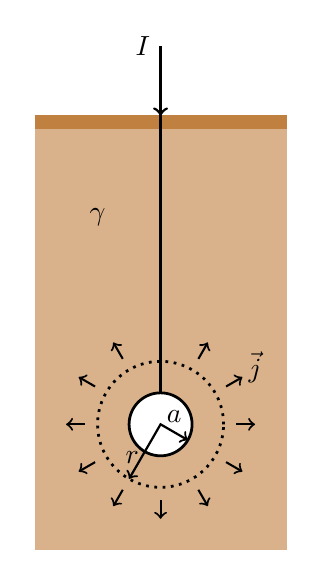
\begin{tikzpicture}[scale=0.8, every node/.style={scale=1}]
      \coordinate (pCenter) at (0,-5);
      \fill[brown!60] (-2,-0.2) rectangle (2,-7);
      \draw[color=brown, line width=5pt] (-2,-0.2) -- +(4,0); 
      \draw[->,line width=1pt] (0,1) node[left] {$I$} -- (0,-0.1);        
      \draw[line width=1pt] (0,0) -- (pCenter);
      \draw[line width=1pt,color=black, fill=white]
           (pCenter) circle[radius=0.5];
      \draw[line width=1pt, dotted]
           (pCenter) circle[radius=1];
      \foreach \angle in
          {0, 30, 60, 120, 150, 180, 210, 240, 270, 300, 330}
      {
        \draw[->, line width=0.75pt] (pCenter)++(\angle:1.2) -- +(\angle:0.3);        
      }
      \draw[<->, thick] (pCenter)++(240:1) coordinate(pR) -- (pCenter) -- +(330:0.5) coordinate(pA); 
      \node[above] at ($ (pCenter)!0.5!(pA) $) {$a$};     
      \node[above] at ($ (pCenter)!0.9!(pR) $) {$r$}; 
      \node[above] at (-1,-2) {$\gamma$};
      \node[above] at (+1.5,-4.5) {$\vec{j}$};
    \end{tikzpicture}
%    \captionsetup{type=figure}
%    \captionof{figure}{Zemnicí elektroda}
%    \label{TEMP:fig_zem_elektroda}
%  \par}
  
\end{document}  